\documentclass[tikz,border=5mm]{standalone}
\usepackage{tikz}
\usetikzlibrary{arrows.meta}
\usepackage{amsmath}
\usepackage{physics}

\ExplSyntaxOn
\msg_redirect_name:nnn { siunitx } { physics-pkg } { none }
\ExplSyntaxOff

\begin{document}
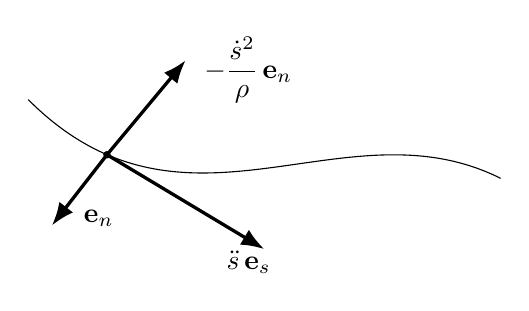
\begin{tikzpicture}[scale=2,
		vector/.style={-{Latex}, very thick}]

    \draw (0, 0.5) .. controls (1, -0.5) and (2, 0.5) ..  (3, 0);
    \draw [fill] (0.5, 0.15) circle (0.02);
    \draw [vector] (0.5, 0.15) -- ++(1, -0.6) node [pos=0.9, below] {$\ddot{s} \, \vb{e}_{s}$};
    \draw [vector] (0.5, 0.15) -- ++(-0.35, -0.45) node [pos=0.9, right=2mm] {$\vb{e}_{n}$};
    \draw [vector] (0.5, 0.15) -- ++(0.5, 0.6) node [pos=0.9, right=2mm] {$-\dfrac{\dot{s}^{2}}{\rho} \, \vb{e}_{n}$};

\end{tikzpicture}
\end{document}